\scanpage{15}
\begingroup
\makeatletter
\tagsleft@true
\makeatother
\uline{\deleted{\unsure{I|V}}Version I}

Soient $X$ un espace topologique, $(\deleted{\unsure{\Sigma|S}}E_i)_{i\in I}$ un ens. de parties \inserted{\unsure{fermés|fermées}} de $X$ (noté indiciellement), telles que l'on ait
% slanted
\reversemarginpar
\margin{$\nearrow$ Supposons de plus que pour \unsure{tte|toute|tt} comp. conn. $\Sigma_{\unsure{i}}$ de $X\setminus E_i$, on ait $\overline{\Sigma}_i\cap E_i\ne\varnothing$ i.e. $\overline{\Sigma}_i\ne\Sigma_i$ i.e. $\Sigma_i$ non fermé dans $X$ (ce qui est le cas si $X$ est \unsure{d.} connexe)}
\normalmarginpar
\[
 \forall i\in I,\quad \operatorname{Card}\unsure{\pi_0|\Pi_0}(X\setminus\deleted{\Sigma}E_i)=2
 \tag*{(a)}
\]
\margin{\uline{NB} les comp. conn. $\Sigma_i^+,\Sigma_i^{\unsure{+|-|\ast}}$ de $X\setminus\Sigma_i$ sont ouvertes dans $X$}
\[
 \begin{aligned}
 &\forall(i,j)\in I\times I,\ i\ne j,\quad \deleted{\Sigma}E_j\ \text{est contenu dans l'une}\\
 &\text{des deux composantes connexes de }X\setminus\deleted{\Sigma}E_i.
 \end{aligned}
 \tag*{(b)}
\]

NB Cette condition (b) est vérifiée \unsure{automatiquement} les $\deleted{\Sigma}E_i$ $(i\in I)$ sont connexes, dès lors que les $E_i$ sont supposés disjoints mutuellement

On se propose d'étudier le ``découpage'' de $X$ par la famille $(E_i)$.

\uline{Cas $\operatorname{Card}\deleted{\unsure{(\mathrm{de})}}(I)\deleted{\unsure{\leq|=}}=2$}

Soit $\Sigma_i^+$ la comp. conn. de $X\setminus E_i$ qui ne contient pas $E_j$ $(j\ne i)$, alors on a (si $I=\{1,2\}$)
\figure{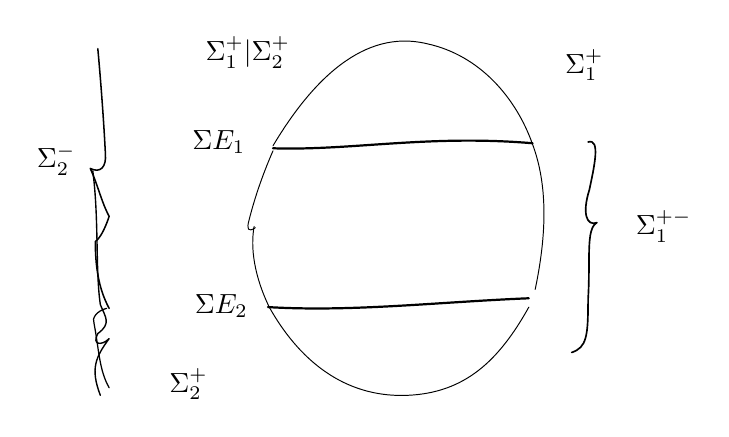
\begin{tikzpicture}[x=.016cm,y=-.016cm,line cap=round,line join=round]
\draw[line width=.35pt] (187,115) .. controls (218,63) and (259,22) .. (309,34)
 .. controls (351,43) and (380,77) .. (393,114)
 .. controls (403,141) and (406,177) .. (395,229);
\draw[line width=.35pt] (390,243) .. controls (366,286) and (339,311) .. (294,313)
 .. controls (249,315) and (211,291) .. (184,243)
 .. controls (172,218) and (169,196) .. (172,179);
\draw[line width=.35pt] (187,119) .. controls (180,135) and (173,154) .. (168,174)
 .. controls (166,181) and (167,184) .. (173,180);
\draw[line width=.8pt] (187,117) .. controls (249,119) and (310,106) .. (393,113);
\draw[line width=.8pt] (183,243) .. controls (250,247) and (317,239) .. (390,236);
\draw[line width=.55pt] (48,38) .. controls (51,71) and (53,101) .. (54,121)
 .. controls (55,132) and (50,137) .. (42,133)
 .. controls (48,146) and (51,160) .. (57,171)
 .. controls (53,183) and (49,189) .. (46,191)
 .. controls (46,215) and (50,231) .. (57,244);
\draw[line width=.5pt] (44,135) .. controls (49,173) and (46,214) .. (50,241)
 .. controls (54,251) and (59,256) .. (48,264)
 .. controls (43,273) and (51,274) .. (57,268)
 .. controls (46,283) and (42,292) .. (50,313);
\draw[line width=.45pt] (55,244) .. controls (47,246) and (43,252) .. (45,256)
 .. controls (49,277) and (49,293) .. (57,307);
\draw[line width=.6pt] (437,112) .. controls (447,109) and (442,131) .. (438,150)
 .. controls (432,169) and (436,179) .. (444,176)
 .. controls (435,181) and (439,205) .. (437,237)
 .. controls (437,266) and (436,275) .. (424,279);
\node at (167,41) {$\deleted{\unsure{\Sigma_1^+|\Sigma_2^+}}$};
\node at (144,112) {$\deleted{\unsure{\Sigma}}E_1$};
\node at (146,242) {$\deleted{\unsure{\Sigma}}E_2$};
\node at (434,51) {$\Sigma_1^+$};
\node at (497,179) {$\Sigma_1^{\deleted{\unsure{+}}\unsure{-}}$};
\node at (15,126) {$\Sigma_2^-$};
\node at (120,304) {$\Sigma_2^+$};
\end{tikzpicture}}
\[
 \Sigma_1^+\cap\Sigma_2^+=\varnothing
 \tag*{(1)}
\]
ce qui \deleted{résulte de}
\[
 \begin{aligned}
 &\deleted{\Sigma_1^-\supset\Sigma_2^+}\qquad\text{\unsure{équivaut à|équiv. à :}}\\
 &\deleted{\Sigma_2^-\supset\Sigma_1^+}\qquad \Sigma_1^+\subset\Sigma_2^-\cup E_2,\quad\text{et}
 \end{aligned}
\]
(\deleted{\unsure{car si}} \deleted{Si on avait} comme $\Sigma_1^+\cap E_2=\varnothing$, cela équivaut aussi à
\[
 \Sigma_1^+\subset\Sigma_2^-
 \tag*{(2)}
\]
\unsure{et} symétriquement, à
\[
 \Sigma_2^+\subset\Sigma_1^-
 \tag*{$(2')$}
\]

Comme \deleted{\unsure{vois. ouvert}} $\Sigma_2^-\supset E_1$, \deleted{il contient les} \inserted{i.e. $\Sigma_2^-$ est un \uline{vois.} ouvert de $E_1$,} on a
% slanted
\reversemarginpar
\margin{$\overline{\Sigma_1^+}\cap E_1\ne\varnothing$ i.e. $\overline{\Sigma_1^+}\ne\Sigma_1^+$ \unsure{à sign.ler|à signaler} avant}
\normalmarginpar
\[
 \Sigma_2^-\cap\Sigma_1^+\ne\varnothing
\]
Car $\underline{\overline{\Sigma_1^+}\cap E_1}\ne\varnothing$ (sinon \inserted{l'ouvert} $\Sigma_1^+$ serait \inserted{\unsure{un|une}} fermé dans $X$, \unsure{puis|donc} \deleted{\unsure{\Sigma_1^+\ne\varnothing|\Sigma_1^+\text{ serait}}} $X$ serait disconnexe),
\endgroup
% archive sheet number: 14
